% Coin toss Bernoulli
\documentclass[tikz = true, border = 2pt]{standalone}
\usepackage{fontspec}
\setmainfont{Equity Text A}
\usepackage{tikz}
\usetikzlibrary{shapes}
\usepackage{xfrac}

\begin{document}
		\begin{tikzpicture}[scale=0.9]
		\node (H) at (0,2) {
			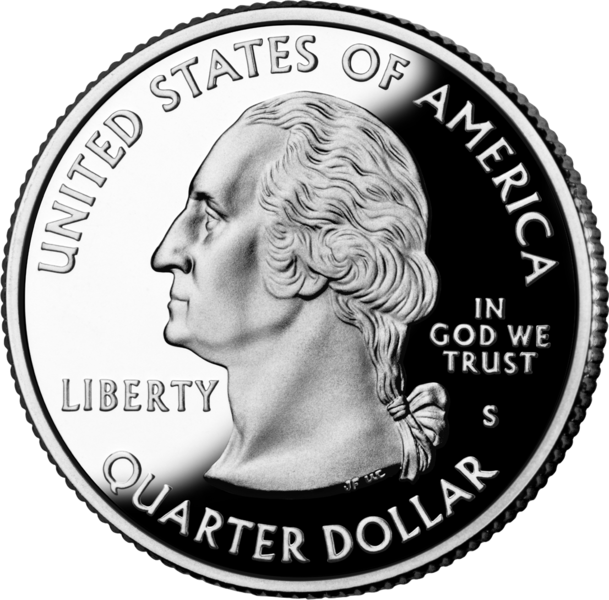
\includegraphics [width=1.5cm]{../images/QuarterHeads.png}
		};
		\node (T) at (0,0) {
			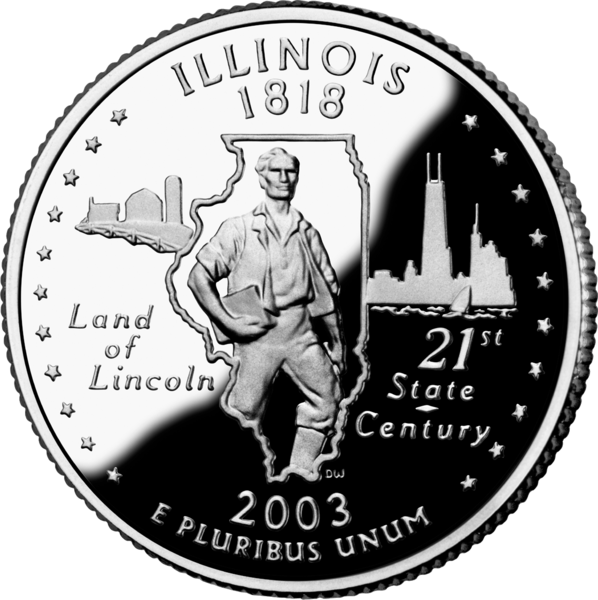
\includegraphics [width=1.5cm]{../images/QuarterTails.png}
		};
		\node [fill=gray!50,
		       minimum height=1.5cm,
		       minimum width=0.1cm,
		       single arrow,
		       single arrow head extend=.15cm,
		       single arrow head indent=.08cm,
		       inner sep=1mm] (arrowtails1) at (1.9,2) {};
		\node [fill=gray!50,
		       minimum height=1.5cm,
		       minimum width=0.1cm,
		       single arrow,
		       single arrow head extend=.15cm,
		       single arrow head indent=.08cm,
		       inner sep=1mm] (arrowheads2) at (1.9,0) {};
		\node  (p1) at (3.4,2) {\huge{$\sfrac{\text{1}}{\text{2}}$}};
		\node  (p2) at (3.4,0) {\huge{$\sfrac{\text{1}}{\text{2}}$}};
		\node [text centered,
		       anchor=south,
		       text height=1.5ex,
		       text depth=.25ex] (p3) at (0,3) {\large{Sample Space}};
		\node [text centered,
		       anchor=south,
		       text height=1.5ex,
		       text depth=.25ex] (p4) at (3.4,3) {\large{Probability}};
		\end{tikzpicture}

\end{document}
